\subtitle{4F13: Machine Learning}
\author[Ghahramani \& Rasmussen]{Zoubin Ghahramani and Carl Edward Rasmussen}
\institute[CUED]{Department of Engineering, University of Cambridge}

\parskip=1.5ex

\newcommand{\maketilde}{\raisebox{0.4ex}{\tiny $\sim$}}
\newcommand{\bfa}{\mathbf a}
\newcommand{\bfb}{\mathbf b}
\newcommand{\bff}{\mathbf f}
\newcommand{\bfm}{\mathbf m}
\newcommand{\bfp}{\mathbf{p}}
\newcommand{\bfs}{\mathbf s}
\newcommand{\bfu}{\mathbf u}
\newcommand{\bfx}{\mathbf x}
\newcommand{\bfy}{\mathbf y}
\newcommand{\bfv}{\mathbf v}

\newcommand{\bmu}{{\boldsymbol{\mu}}}
\newcommand{\btheta}{\boldsymbol{\theta}}
\newcommand{\balpha}{\boldsymbol{\alpha}}
\newcommand{\bphi}{\boldsymbol{\phi}}
\newcommand{\bpi}{\boldsymbol{\pi}}
\newcommand{\blambda}{\boldsymbol{\lambda}}

\newcommand{\N}{\mathcal{N}}
\newcommand{\R}{\mathbb{R}}
\newcommand{\T}{{\scriptsize^{\top}}}
\newcommand{\D}{\mathcal{D}}
\newcommand{\F}{\mathcal{F}}
\newcommand{\E}{\mathbb{E}}
\newcommand{\V}{\mathbb{V}}
\newcommand{\M}{\mathcal{M}}
\newcommand{\KL}{\mathcal{KL}}
\newcommand{\cut}[1]{}
\newcommand{\trace}{\operatorname{trace}}

\newcommand{\argmax}{\operatorname{argmax}}
\newcommand{\argmin}{\operatorname{argmin}}
\newcommand{\ci}{{\bot\negthickspace\negthickspace\bot}} % conditional indep.
\newcommand{\neigh}{\operatorname{ne}}
\newcommand{\vectr}[2]{  \left[ \!\!\begin{array}{c} #1 \\
      #2 \end{array} \!\!\right]}
\newcommand{\deff}{\stackrel{\mathrm{def}}{=}}
\newcommand{\deldel}[2]{\frac{\partial #1}{\partial #2}}


\definecolor{mypine}{rgb}{0.05,0.45,0.05}
\definecolor{mycyan}{rgb}{0.0,0.4,0.4}
\newcommand{\Red}{\textcolor{red}}
\newcommand{\Blue}{\textcolor{blue}}
\newcommand{\Green}{\textcolor{mypine}}
\newcommand{\PineGreen}{\textcolor{mypine}}
\newcommand{\Magenta}{\textcolor{magenta}}


\begin{document}

\titleslide{Lecture 7: Markov Chain Monte Carlo}{February 8th and 13th, 2008}

\begin{frame}
\frametitle{Objective}

Approximate \Blue{expectations} of a function $\phi(\bfx)$ wrt
\Blue{probability} $p(\bfx)$:
\[
\E_{p(x)}[\phi(x)]\;=\;\bar\phi\;=\;\int \phi(\bfx)\Red{p(\bfx)}d\bfx,
\text{\ \ where\ \ }\bfx\in\R^D,
\]
when these are not analytically tractable, and typically $D\gg1$.
\begin{center}
\includegraphics[width=0.8\textwidth]{mc0}
\end{center}
Assume that we can evaluate $\phi(x)$ and $\Red{p(x)}$, or at least
$\Red{p^*(x)}$, an un-normalized version of $\Red{p(x)}$, for any value of $x$.
\end{frame}

\begin{frame}
\frametitle{Motivation}

Such integrals, or marginalizations, are \Blue{essential for probabilistic
inference and learning}:
\begin{itemize}
\item Making predictions, e.g. in supervised learning
\[
p(y_*|x_*,\D)\;=\;\int p(y_*|x_*,\theta)\Red{p(\theta|\D)}d\theta,
\]
where the \emph{posterior distribution} playes the rôle of $\Red{p(x)}$
\item Approximate marginal likelihoods
\[
p(\D|\M_i)\;=\;\int p(\D|\theta,\M_i)\Red{p(\theta|\M_i)}d\theta,
\]
where the \emph{prior distribution} playes the rôle of $\Red{p(x)}$.
\end{itemize}
\end{frame}

\begin{frame}
\frametitle{Numerical integration on a grid}

Approximate the integral by a sum of products
\[
\int \phi(\bfx)\Red{p(\bfx)}d\bfx\;\simeq\;\frac{1}{T}\sum_{\tau=1}^T\phi(\bfx^{(\tau)})\Red{p(\bfx^{(\tau)})},
\]
where the $\bfx^{(\tau)}$ lie on an equidistant grid (or fancier
versions of this).
\begin{center}
\includegraphics[width=0.8\textwidth]{mc1}
\end{center}
\Blue{Problem:} the number of grid points required, $k^D$, grows
exponentially with the dimension $D$.
\end{frame}

\begin{frame}
\frametitle{Monte Carlo}

The foundation identity for Monte Carlo approximations is
\[
\E[\phi(\bfx)]\;\simeq\;\hat\phi\;=\;\frac{1}{T}\sum_{\tau=1}^T\phi(\bfx^{(\tau)}).
\text{\ \ where\ \ }\bfx^{(\tau)}\sim \Red{p(\bfx)}.
\]
Under mild conditions, $\hat\phi\rightarrow\E[\phi(\bfx)]$ as
$T\rightarrow\infty$.

For moderate $T$, $\hat\phi$ may still be a good approximation. In
fact it is an \emph{unbiased} estimate with
\[
\V[\hat\phi]\;=\;\frac{\V[\phi]}{T}, \text{\ \ where\ \ }
\V[\phi]\;=\;\int \big(\phi(\bfx)-\bar\phi\big)^2\Red{p(\bfx)}d\bfx.
\]
\Blue{Note}, that this variance in \Blue{independent} of the dimension
$D$ of $\bfx$.

This is great, but \Blue{how do we generate random samples} from
$\Red{p(\bfx)}$?
\end{frame}

\begin{frame}
\frametitle{Random number generation}

There are (pseudo-) random number generators for the uniform $[0; 1]$
distribution.

Transformation methods exist to turn these into other simple
univariate distributions, such as Gaussian, Gamma, \ldots, as well as some
multivariate distributions e.g. Gaussian and Dirichlet.

\Blue{Example}: $p(x)$ is uniform $[0; 1]$. The transformation $y=-\log(x)$
yields:
\[
p(y)\;=\;p(x)\big|\frac{dx}{dy}\big|\;=\;\exp(-y),
\]
i.e. an \emph{exponential} distribution.

Typically $\Red{p(\bfx)}$ may be more complicated.

How can we generate samples from a (multivariate) distribution $\Red{p(\bfx)}$?

\Blue{Idea}: we can discretize $\Red{p(\bfx)}$, and sample from the
discrete \Blue{multinomial} distribution. Will this work?
\end{frame}

\begin{frame}
\frametitle{Rejection sampling}

Find a tractable distribution $\Blue{q(\bfx)}$ and $c\geq 1$, such that $\forall\bfx, c\Blue{q(\bfx)}\geq\Red{p(\bfx)}$.
\begin{center}
\includegraphics[width=0.8\textwidth]{mc2}
\end{center}
Rejection sampling algorithm:
\begin{itemize}
\item Generate samples independently from $\Blue{q(\bfx)}$
\item Accept samples with probability $\Red{p(\bfx)}/(c\Blue{q(\bfx)})$, otherwise reject
\item Form a Monte Carlo estimate from the accepted samples.
\end{itemize}
This estimate with be \Blue{exactly unbiased}. How effective will it be?
\end{frame}

\begin{frame}
\frametitle{Importance sampling}

Find a tractable $\Blue{q(\bfx)}\simeq\Red{p(\bfx)}$, such that
$\Blue{q(\bfx)}>0$ whenever $\Red{p(\bfx)}>0$.
\begin{center}
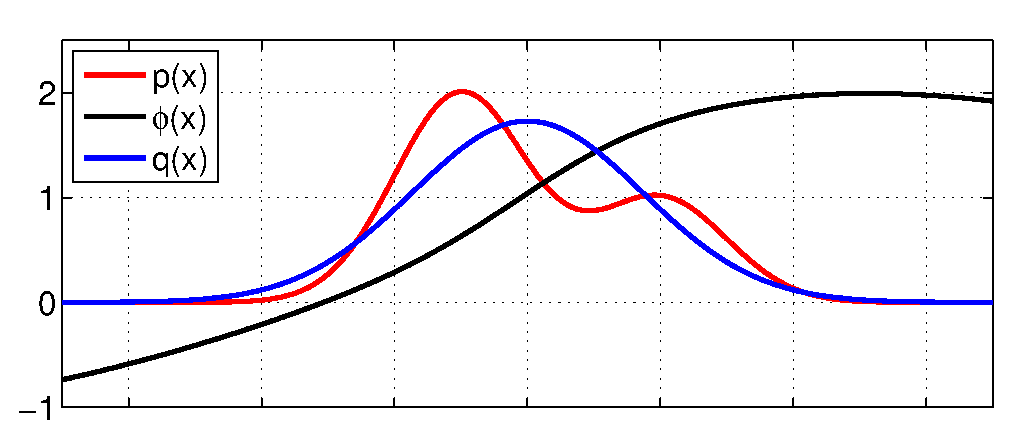
\includegraphics[width=0.8\textwidth]{mc3}
\end{center}
Form the Importance sampling estimate:
\[
\int \phi(\bfx)\frac{\Red{p(\bfx)}}{\Blue{q(\bfx)}}\Blue{q(\bfx)}d\bfx\;
\simeq\;\hat\phi\;=\;\frac{1}{T}\sum_{\tau=1}^T\phi(\bfx^{(\tau)})
\underset{w(\bfx^{(\tau)})}{\underbrace{\frac{\Red{p(\bfx^{(\tau)})}}{\Blue{q(\bfx^{(\tau)})}}}}, \text{\ \ where\ \ }
x^{(\tau)}\sim\Blue{q(\bfx)},
\]
where $w(\bfx^{(\tau)})$ are called the \emph{importance weights}.
\end{frame}

\begin{frame}
There is also a version of importance sampling which doesn't require knowing
how $\Blue{q({\bfx})}$ normalizes:
\[
\hat\phi\;=\;\frac{\sum_\tau\phi(\bfx^{(\tau)})w(\bfx^{(\tau)})}{\sum_\tau w(\bfx^{(\tau)})}, \text{\ \ where\ \ }w(\bfx^{(\tau)})=\frac{\Red{p(x^{(\tau)})}}{\Blue{q^*(\bfx^{(\tau)})}}, \text{\ \ and\ \ }\bfx^{(\tau)}\sim\Blue{q(\bfx)}.
\]

How fast is importance sampling? This depends on the variance of the importance
weights.

{\bf Example}: $\Red{p(x)=\N(0,1)}$ and $\Blue{q(x)=\N(0,\sigma^2)}$. The
variance of the weights is:
\[
\begin{split}
\V[w]\;=\;\E[w^2]-\E^2[w]\;&=\;\int\frac{p(x)^2}{q(x)^2}q(x)dx-\Big(\int\frac{p(x)}{q(x)}q(x)dx\Big)^2\\
&=\;\sigma\int\exp(-x^2+\frac{x^2}{2\sigma^2})dx-1.
\end{split}
\]
which only exists when $\sigma>\sqrt{1/2}$. Morale: always chose $q(\bfx)$ to
be wider, have `heavier tails' than $p(\bfx)$ to avoid this problem.
\end{frame}

\begin{frame}
\frametitle{Rejection and Importance sampling}

In the multivariate case with Gaussian $\Blue{q(\bfx)}$ we must be able to
guarantee that no direction exist when we underestimate the width by more than
a factor of $\sqrt{2}$.

In fact, both rejection and importance sampling have severe problems in high
dimensions, since it is virtually impossible to get $\Blue{q(\bfx)}$ close
enough to $\Red{p(\bfx)}$, see MacKay chapter 29 for details.
\end{frame}

\begin{frame}
\frametitle{Independent Sampling vs.~Markov Chains}

So far, we've considered two methods, Rejection and Importance
Sampling, which were both based on independent samples from $\Blue{q(\bfx)}$.

However, for many problems of practical interest it is difficult or
impossible to find $q(\bfx)$ with the necessary properties.

Instead we can abandon the idea of independent sampling, and instead
rely on a \Blue{Markov Chain} to generate \Blue{dependent} samples
from the target distribution.

\Blue{Independence} would be a nice thing, but it is not necessary for
the Monte Carlo estimate to be valid.
\end{frame}

\begin{frame}
\frametitle{Markov Chain Monte Carlo}

We want to construct a Markov Chain that explores $\Red{p(\bfx)}$.

Markov Chain: $\bfx^{(t)}\sim q(\bfx^{(t)}|\bfx^{(t-1)})$.
\begin{center}
\includegraphics[width=0.6\textwidth]{mcmc}
\end{center}
MCMC gives \Red{approximate}, \Red{correlated} samples from $p(x)$.

\Blue{Challenge:} how do we find \Blue{transition probabilities}
$q(\bfx^{(t)}|\bfx^{(t-1)})$, which give rise to the correct
\Blue{stationary distribution} $p(\bfx)$?
\end{frame}

\begin{frame}
\frametitle{Discrete Markov Chains}

Consider
\[
{\bf p}\;=\;\left[\begin{array}{c}3/5\\1/5\\1/5\end{array}\right],\qquad
Q\;=\;\left[\begin{array}{ccc}2/3&1/2&1/2\\ 1/6&0&1/2\\ 1/6&1/2&0\end{array}
\right],\qquad
Q_{ij}\;=\;Q(x_i\leftarrow x_j)
\]
where $Q$ is a stochastic (or transition) matrix.

To machine precision: $Q^{100}\left[\begin{array}{c}1\\0\\0\end{array}\right]={\bf p}$.

${\bf p}$ is called a \Blue{stationary distribution} of $Q$, since $Q{\bf p}={\bf p}$.

Ergodicity is also a requirement. 
\end{frame}

\begin{frame}
\frametitle{In Continuous Spaces}

In continuous spaces transitions are governed by $q(\bfx'|\bfx)$.

Now, $p(\bfx)$ is a stationary distribution for $q(\bfx'|\bfx)$ if
\[
\int q(\bfx'|\bfx)p(\bfx)d\bfx\;=\;p(\bfx').
\]
\end{frame}


\begin{frame}
\frametitle{Detailed Balance}

\Blue{Detailed balance} means
\[
q(\bfx'|\bfx)p(\bfx)\;=\;q(\bfx|\bfx')p(\bfx').
\]

Now, integrating both sides wrt $\bfx$, we get
\[
\int q(\bfx'|\bfx)p(\bfx)d\bfx\;=\;\int q(\bfx|\bfx')p(\bfx')d\bfx\;=\;p(\bfx').
\]

Thus, \Blue{detailed balance} implies the existence of a
\Blue{stationary distribution}
\end{frame}


\begin{frame}
\frametitle{The Metropolis-Hastings algorithm}

The Metropolis-Hastings algorithm:
\begin{itemize}
\item propose a new state $\bfx^*$ from $q(\bfx^*|\bfx^{(\tau)})$
\item compute the \Blue{acceptance probability} $a$
\[
a\;=\;\frac{p(\bfx^*)}{p(\bfx^{(\tau)})}
\frac{q(\bfx^{(\tau)}|\bfx^*)}{q(\bfx^*|\bfx^{(\tau)})}
\]
\item if $a>1$ then the proposed state is accepted,\\
otherwise the proposed state is accepted with probability $a$.\\
If the proposed state is accepted,
  then $\bfx^{(\tau+1)}=\bfx^*$ otherwise $\bfx^{(\tau+1)}=\bfx^{(\tau)}$.
\end{itemize}
This Markov chain has $p(\bfx)$ as a stationary distribution. This
holds trivially if $\bfx^{(\tau+1)}=\bfx^{(\tau)}$, otherwise
\[
\begin{split}
p(\bfx)Q(\bfx'\leftarrow\bfx)\;&=\;p(\bfx)q(\bfx'|\bfx)\min\Big(1,\frac{p(\bfx')q(\bfx|\bfx')}{p(\bfx)q(\bfx'|\bfx)}\Big)\\
&=\;\min\big(p(\bfx)q(\bfx'|\bfx),p(\bfx')q(\bfx|\bfx')\big)\\
&=\;p(\bfx')q(\bfx|\bfx')\min\Big(1,\frac{p(\bfx)q(\bfx'|\bfx)}{p(\bfx')q(\bfx|\bfx')}\Big)\;=\;p(\bfx')Q(\bfx\leftarrow\bfx').
\end{split}
\]
\end{frame}

\begin{frame}
\frametitle{Some properties of Metropolis Hastings}

\begin{itemize}
\item The Metropolis algorithm has $p(\bfx)$ as its stationary distribution
\item If $q(\bfx^*|\bfx^{(\tau)})$ is symmetric, then
  \begin{itemize}
\item the expression for $a$ simplifies to
    $a=p(\bfx^*)/p(\bfx^{(\tau)})$
\item the algorithm then always accepts if the proposed state has higher
probability than the current state and sometimes accepts a state with
lower probability.
\end{itemize}
\item  we only need the ratio of $p(\bfx)$'s, so we don't need the
normalization constant. This is important, e.g. when sampling from a 
posterior distribution.
\end{itemize}

The Metropolis algorithm can be widely applied, you just need to specify 
a proposal distribution.

The proposal distribution must satisfy some (mild) constraints
(related to ergodicity).

\end{frame}

\begin{frame}
\frametitle{The Proposal Distribution}

Often, Gaussian proposal distributions are used, centered on the current state.
You need to specify the width of the proposal distribution.

What happens if the proposal distribution is
\begin{itemize}
\item too wide?
\item too narrow?
\end{itemize}
\end{frame}

\begin{frame}
\frametitle{Metropolis Hastings Example}

20 iterations of the Metropolis Hastings algorithm for a bivariate Gaussian
\begin{center}
\includegraphics[width=0.4\textwidth]{bvg-metrop}
\end{center}
The proposal distribution was Gaussian centered on the current state.

Rejected states are indicated by dotted lines.
\end{frame}


\begin{frame}
\frametitle{Random walks}

When exploring a distribution with the Metropolis algorithm, the proposal has
to be narrow to avoid too many rejections.

If a typical step moves a distance $\varepsilon$, then one needs an expected
$T=(L/\varepsilon)^2$ steps to travel a distance of $L$. This is a problem with
random walk behavior.

Notice that \Blue{strong correlations} can \Blue{slow down} the Metropolis
algorithm, because the proposal width should be set according to the tightest
direction.
\end{frame}

\begin{frame}
\frametitle{Variants of the Metropolis algorithm}

Instead of proposing a new state by changing simultaneously all
components of the state, you can concatenate different proposals
changing one component at a time.

For example, $q_j(\bfx'|\bfx)$, such that $x'_i=x_i,\,\forall i\neq j$.

Now, cycle through the $q_j(\bfx'|\bfx)$ in turn.

This is valid as
\begin{itemize}
\item each iteration obeys detailed balance
\item the \emph{sequence} guarantees ergodicity
\end{itemize}
\end{frame}

\begin{frame}
\frametitle{Gibbs sampling}

Updating one coordinate at a time, and choosing the proposal
distribution to be the conditional distribution of that variable given
all other variables $\Blue{q(x'_i|\bfx)=p(x'_i|x_{\neq i})}$ we get
\[
a\;=\;\min\Big(1,\frac{p(x_{\neq i})p(x'_i|x_{\neq i})\Blue{p(x_i|x'_{\neq i})}}
{p(x_{\neq i})p(x_i|x_{\neq i})\Blue{p(x'_i|x_{\neq i})}}\Big)\;=\;1,
\]
i.e., we get an \Blue{algorithm which always accepts}. This is called
the Gibbs sampling algorithm.

If you can compute (and sample from) the conditionals, you can apply Gibbs
sampling.

This algorithm is completely parameter free.

Can also be applied to subsets of variables.
\end{frame}

\begin{frame}
\frametitle{Example: Gibbs Sampling}

20 iterations of Gibbs sampling on a bivariate Gaussian
\begin{center}
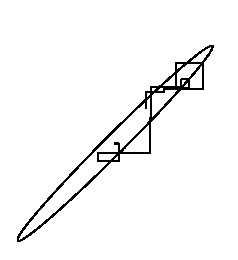
\includegraphics[width=0.4\textwidth]{bvg-gibbs}
\end{center}

Notice that \Blue{strong correlations} can \Blue{slow down} Gibbs sampling.
\end{frame}

\begin{frame}
\frametitle{Hybrid Monte Carlo}

Define a joint distribution over position and velocity
\begin{itemize}
\item $p(\bfx,\bfv)=p(\bfv)p(\bfx)=e^{-E(\bfx)-K(\bfv)}=e^{-H(\bfx,\bfv)}$.
\item $\bfv$ independent of $\bfx$ and $\bfv\sim{\cal N}(0,1)$.
\item sample in the joint space, then ignore the velocities to get the
  positions.
\end{itemize}

Markov chain:
\begin{itemize}
\item Gibbs sample velocities using ${\cal N}(0,1)$
\item Simulate Hamiltonian dynamics through fictitious time, then
  negate velocity
\begin{itemize}
\item 'proposal' is deterministic and reversible
\item conservation of energy guarantees $p(\bfx,\bfv)=p(\bfx',\bfv')$
\item Metropolis acceptance probability is 1.
\end{itemize}
\end{itemize}
\Blue{But we can not usually simulate Hamiltonian dynamics exactly.}
\end{frame}

\begin{frame}
\frametitle{Leap-frog dynamics}

a discrete approximation of Hamiltonian dynamics:
\[
\begin{split}
v_i(t+\tfrac{\varepsilon}{2})\;&=\;v_i(t)-\frac{\varepsilon}{2}\frac{\partial E(\bfx(t))}{\partial x_i}\\
x_i(t+\varepsilon)\;&\;x_i(t)+\varepsilon v_i(t+\tfrac{\varepsilon}{2})\\
v_i(t+\varepsilon)\;&=\;v_i(t+\tfrac{\varepsilon}{2})-\frac{\varepsilon}{2}\frac{\partial E(\bfx(t+\varepsilon))}{\partial x_i}
\end{split}
\]
\begin{itemize}
\item using $L$ steps of Leap-frog dynamics
\item $H$ is no-longer exactly conserved
\item dynamics still deterministic and reversible
\item acceptance probability $\min(1,\exp(H(\bfv,\bfx)-H(\bfv',\bfx')))$
\end{itemize}
\end{frame}

\begin{frame}
\frametitle{Hybrid Monte Carlo avoids random walks}

\begin{center}
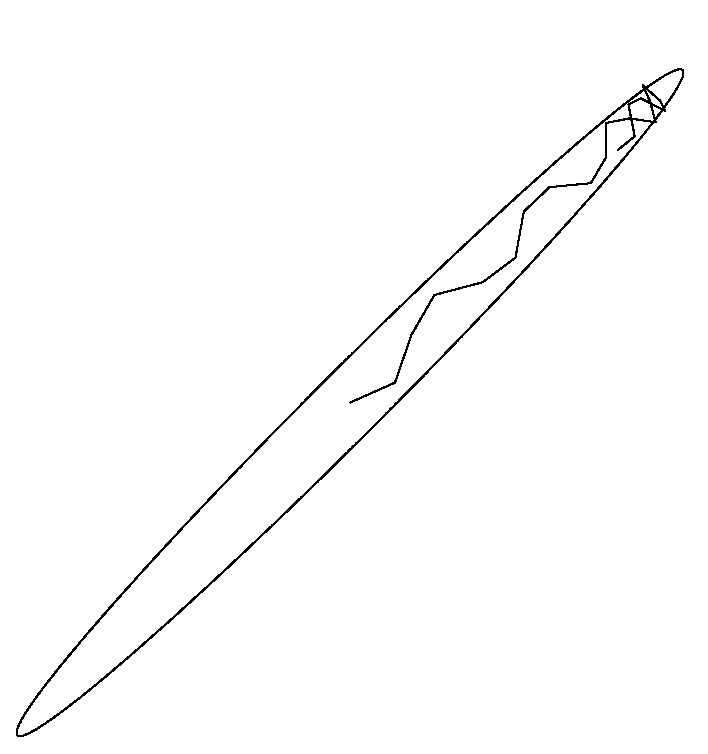
\includegraphics[width=0.4\textwidth]{bvg-hybrid}
\end{center}

The advantage of introducing velocity variables is that random walks
are avoided.

\end{frame}


\begin{frame}
\frametitle{Summary}

Rejection and Importance sampling are based on independent samples from
$\Blue{q(\bfx)}$.

These methods are not suitable for high dimensional problems.

The Metropolis method, does not give independent samples, but can be used
successfully in high dimensions.

Gibbs sampling is used extensively in practice.
\begin{itemize}
\item parameter-free
\item requires simple conditional distributions
\end{itemize}

Hybrid Monte Carlo is used extensively in continuous systems
\begin{itemize}
\item avoids random walks
\item requires setting of $\varepsilon$ and $L$.
\end{itemize}
\end{frame}

\begin{frame}
\frametitle{Monte Carlo in Practice}

Although very general, and can be applied in systems with 1000's of
variables.

Care must be taken when using MCMC
\begin{itemize}
\item high dependency between variables may cause slow exploration
\begin{itemize}
\item how long does 'burn-in' take?
\item how correlated are the samples generated?
\item \Blue{slow} exploration may be hard to detect -- but you might
  not be getting the right answer
\end{itemize}
\item diagnosing a convergence problem may be difficult
\item curing a convergence problem may be even more difficult
\end{itemize}
\end{frame}

\end{document}